\chapter{Procesos para presentaci\'on de proyectos}

Vicerector\'ia de investigaciones de la Universidad de la Amazonia cuenta con una serie de procesos determinados para la propuesta y aceptaci�n de proyectos de investigaci�n, generalmente estos �ltimos provienen de docentes, grupos y/o semilleros de investigaci�n.
\\

Actualmente, existen 3 formas de presentar proyectos, estas son como: semillero, grupo y docente, este ultimo conocido como iniciativa propia. Los proyectos presentados por parte de los semilleros y grupos de investigaci�n obedecen a una convocatoria, es decir, el mismo proceso a seguir para los dos [ver figura \ref{proc_proy_grup_sem_inv}]. El caso es diferente para aquellos que se incluyen dentro del marco de iniciativa propia [ver figura \ref{proc_proy_inv_ini_doc}].

\section{Presentaci�n de propuesta de proyecto: Docente}

El proceso de presentaci�n y evaluaci�n de proyectos de iniciativa propia (docente) empiezan por una propuesta de investigaci�n, la cual es llevada a cabo por una serie de formatos que posteriormente son evaluados por instancias de la misma universidad, estas corresponden a: comit� de curr�culo, consejo de facultad, comit� de investigaciones y vicerector�a de investigaciones, siendo este el orden de evaluaci�n respectivamente. Aqu� se determina la viabilidad de la propuesta, llegado el caso en que no sea factible se procede a devoluci�n.
\\ 

Cuando una propuesta es aceptada (es factible), se asigna un plan de trabajo que ser� ejecutado, seguido y evaluado por un par evaluador hasta llegar al cierre del mismo, ver imagen \ref{proc_proy_inv_ini_doc}.
\\

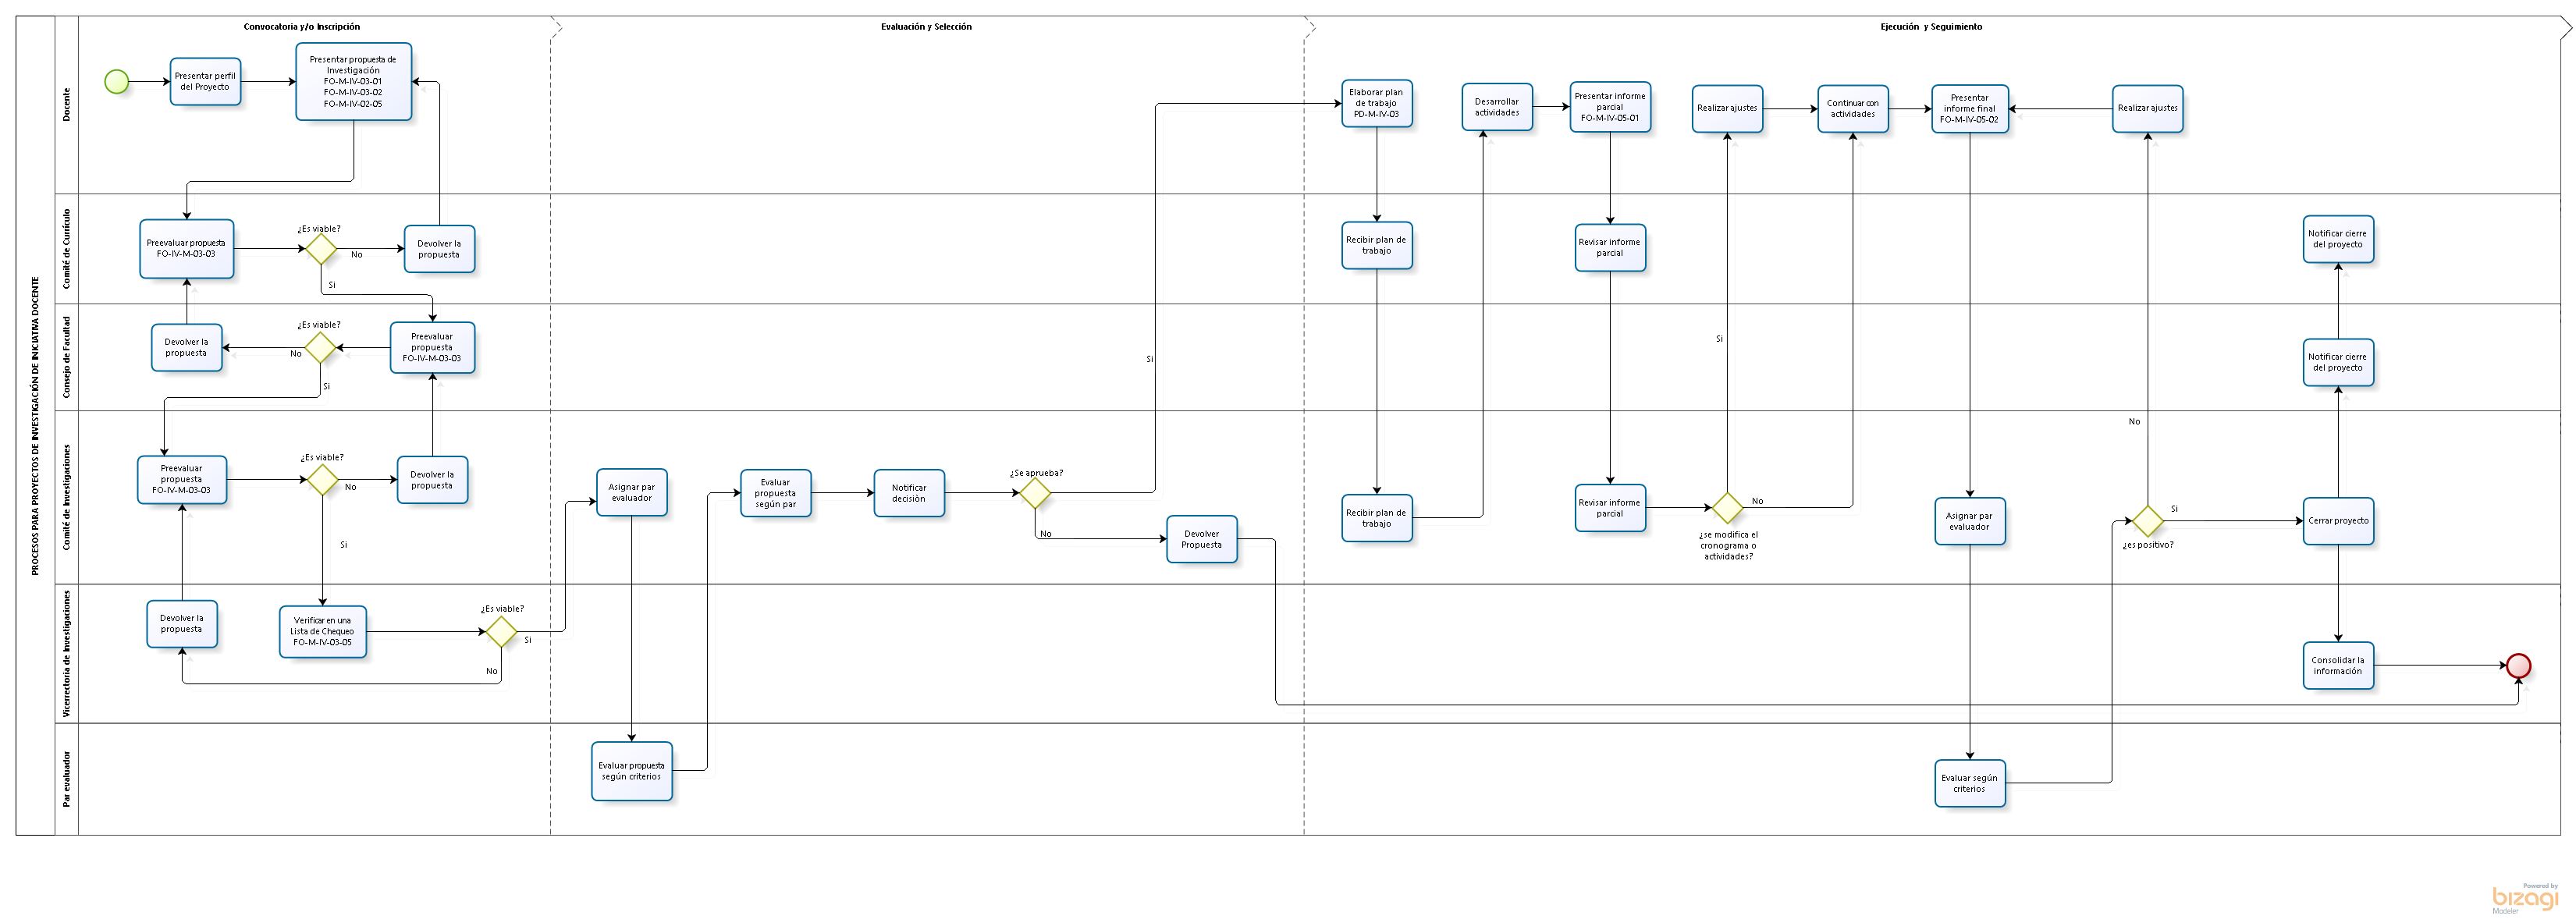
\includegraphics[width=\textwidth]{resources/procesos/PROPUESTO_INICIATIVA_DOCENTE.PNG} %
\captionof{figure}{Procesos para proyectos de investigaci�n iniciativa docente}
\label{proc_proy_inv_ini_doc}

\section{Presentaci�n de propuesta de proyecto: Grupos y semilleros de investigaci�n}

A diferencia de la propuesta docente, los grupos y semilleros deben empezar por la presentaci�n de la propuesta a vicerector�a de investigaciones, consejo superior se encarga de evaluarla y aprobarla, luego de tramitar los formatos para presentaci�n de propuestas de investigaci�n el par evaluador asignado procede con la evaluaci�n teniendo en cuenta criterios determinados, luego este pasa a ejecuci�n y seguimiento. 
\\

El plan de ejecuci�n y seguimiento tiene como objetivo la vigilancia del cumplimiento de cada actividad propuesta en el plan de trabajo inicial, estas son revisadas mediante un informe parcial hasta finalmente concluir en un informe final que conlleva al exitoso cierre y consolidaci�n del proyecto, ver imagen [\ref{proc_proy_grup_sem_inv}].
\\

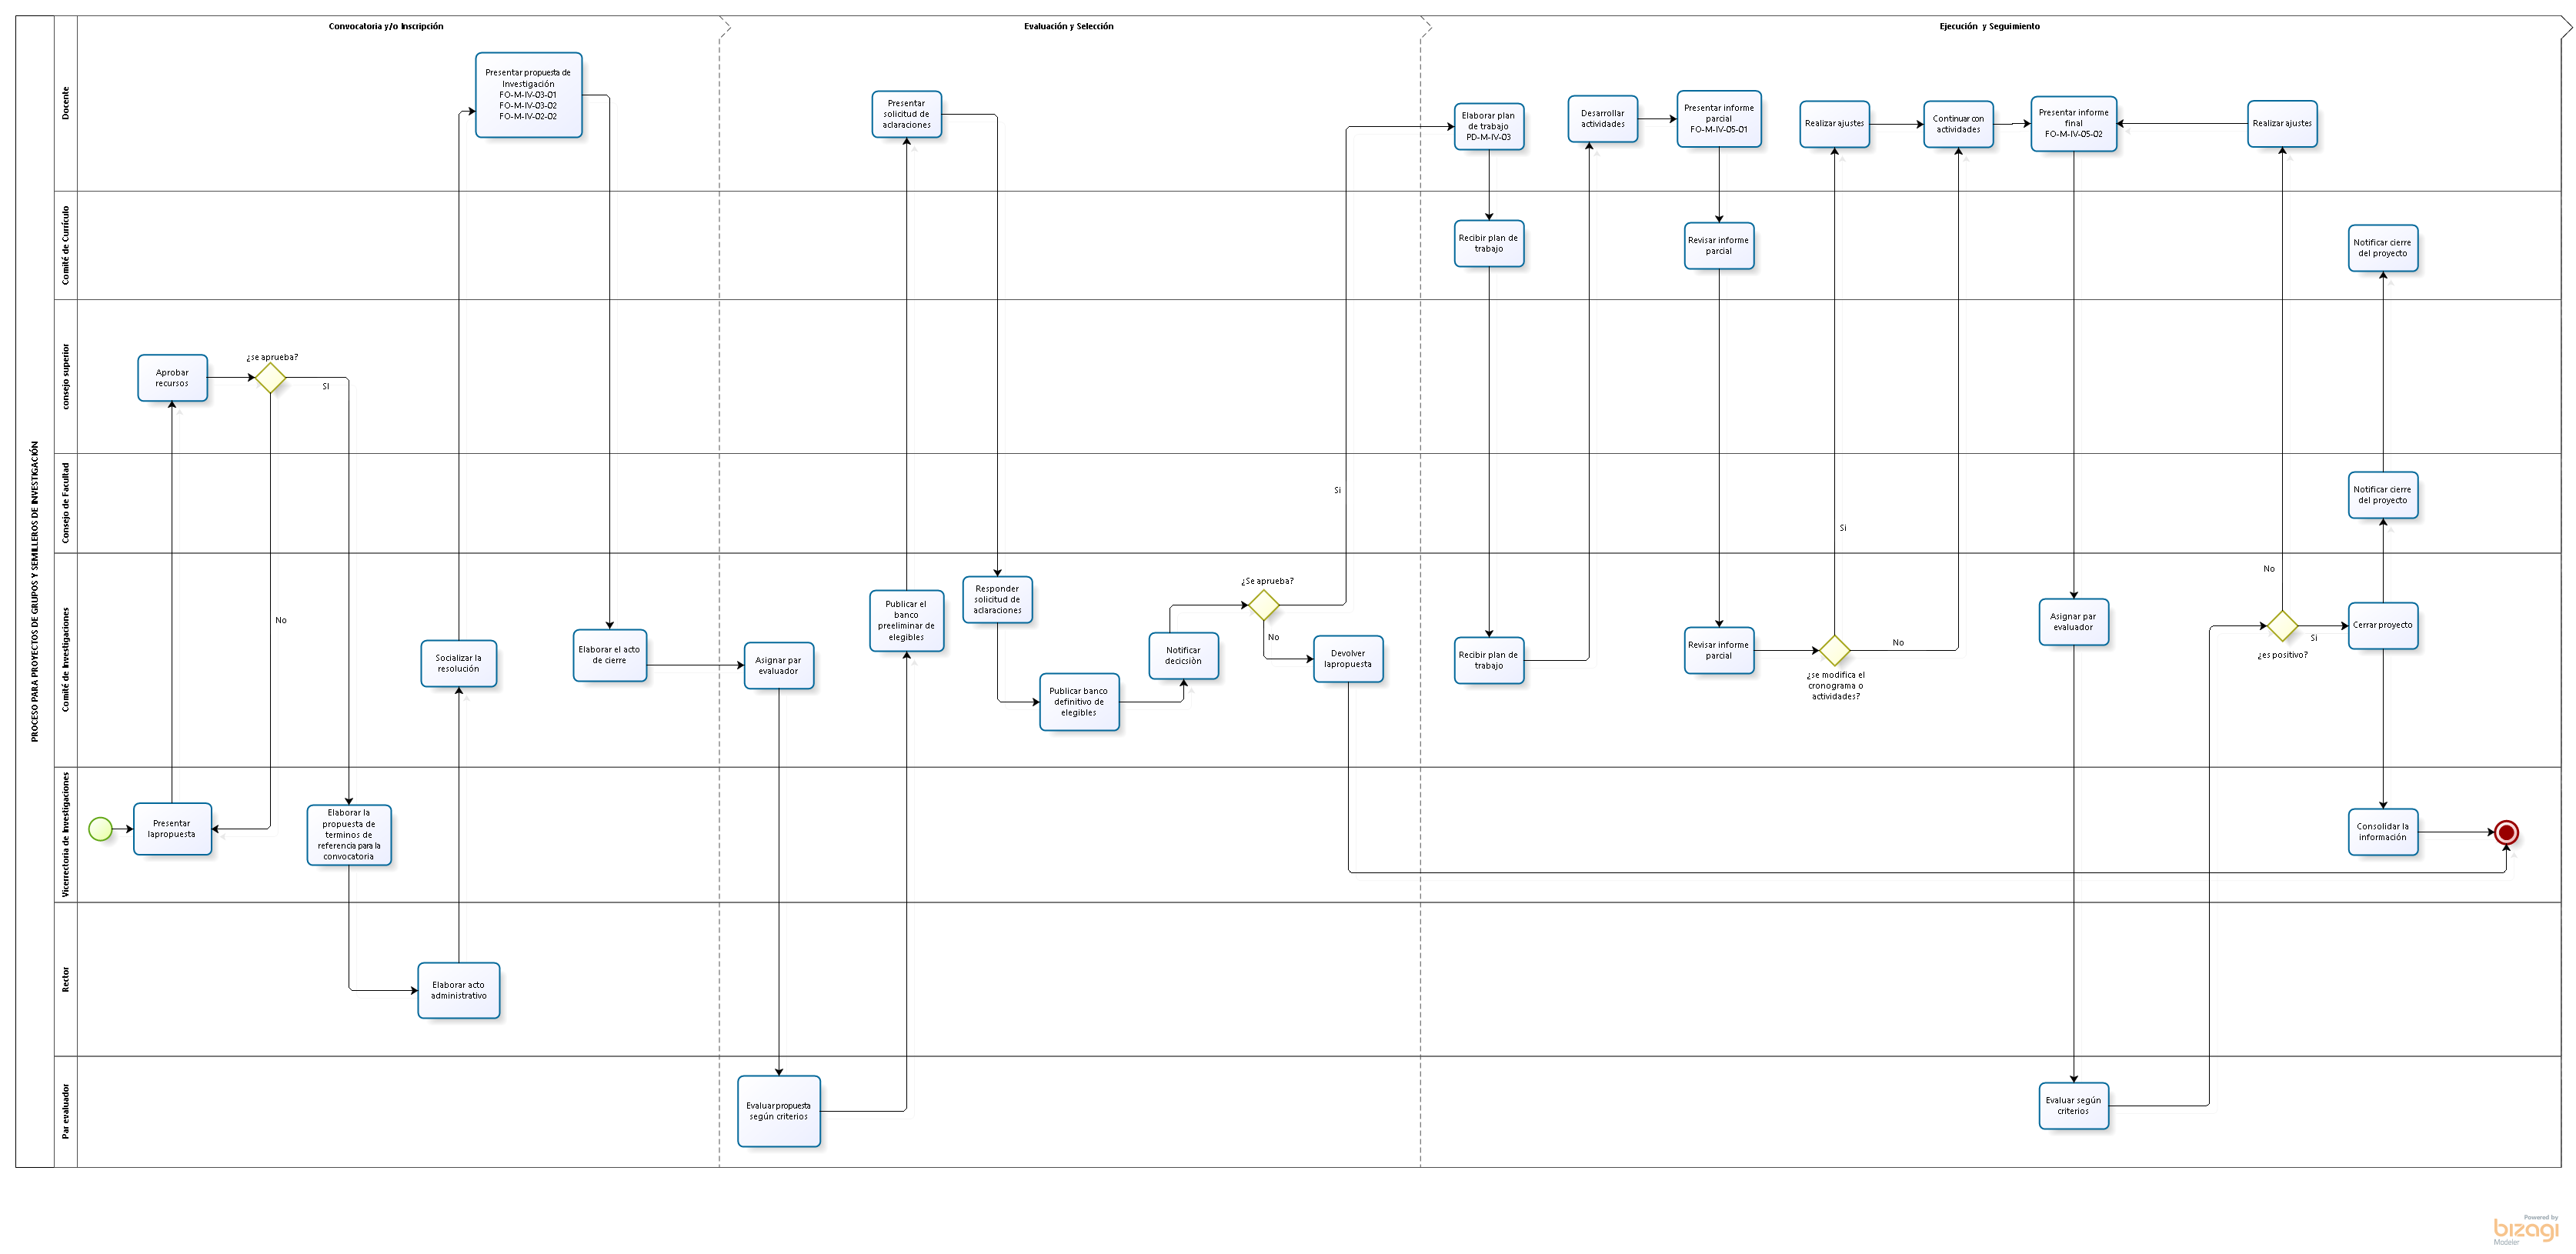
\includegraphics[width=\textwidth]{resources/procesos/PROPUESTA_CONVOCATORIA_GRUPOS_SEMILLEROS.PNG} %
\captionof{figure}{Procesos para proyectos de grupos y semilleros de investigaci�n}
\label{proc_proy_grup_sem_inv}